% =====================================================================
\section{Visual Demonstrations (MuJoCo and Browser)}
\label{sec:demos}
% =====================================================================

These demos make the controller \emph{visible}; the quantitative evidence is in \cref{sec:repro,sec:beyond,sec:x3res}.

\subsection{MuJoCo: two bodies side by side}

\code{Drones\_Mujoco\_Pointing\_Trial.ipynb} integrates the paper's equations for two rigid bodies in MuJoCo's 3-D viewer:
the left (blue) one runs the constrained PD-type law (paper barrier form), the right (orange) one conventional PD. Three
demos are included: the paper's Part~2 manoeuvre, turning to any attitude entered as roll/pitch/yaw, and pointing the nose
at a target position (each body's dotted line of sight reaches the gold target only when it is truly aimed at it). The
notebook sizes $\rho_{q0}$ from the requested rotation so that the initial state is strictly inside the envelope
(e.g.\ $\rho_{q0}=0.367$ for a $30^\circ/30^\circ/30^\circ$ target, $1.057$ for the large pointing turn).

\begin{figure}[H]
\centering
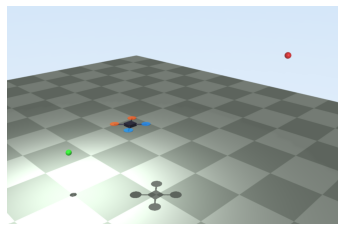
\includegraphics[width=0.46\linewidth]{mujoco_pointing_cell1.png}\hfill
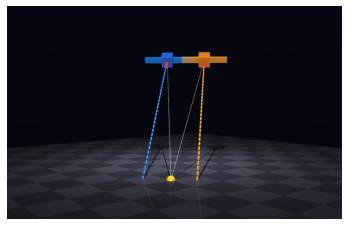
\includegraphics[width=0.46\linewidth]{mujoco_pointing_cell9.png}
\caption{MuJoCo scenes from the notebook: a quadrotor-shaped body flying to a goal (left) and the two bodies pointing their
lines of sight at a target (right).}
\label{fig:mujocoviews}
\end{figure}

\begin{toybox}[printed output of the Part-2 demo, $\|\qv\|$ every second]
\small
\begin{tabular}{@{}lcccccccccc@{}}
$t$ (s) & 0 & 1 & 2 & 3 & 4 & 5 & 6 & 7 & 8 & 9\\
constrained & 0.469 & 0.401 & 0.240 & 0.128 & 0.067 & 0.036 & 0.017 & 0.009 & 0.005 & 0.002\\
conventional PD & 0.469 & 0.401 & 0.214 & 0.031 & 0.048 & 0.040 & 0.016 & 0.003 & 0.007 & 0.006
\end{tabular}

The constrained body decays monotonically (no overshoot through zero); the PD body is sometimes ahead and then swings past
zero and back ($0.031\to0.048$). $\|\qv\|$ alone does not show the envelope, which is why the reproduction reports
$|\varepsilon|$ and the time outside (\cref{sec:part2}).
\end{toybox}

\subsection{MuJoCo: flight with altitude and attitude loops}

\code{Drones\_Mujoco\_Flying.ipynb} and \code{Drones\_Mujoco\_Good\_Trial.ipynb} add an altitude/position loop around the
attitude law on a quadrotor-shaped body with direct force and torque actuators (not four-rotor mixing).

\resfig{mujoco_flying_cell5.png}{0.6\linewidth}{MuJoCo flight: climb to 2\,m while the attitude quaternion converges from the
paper's Part-1 initial attitude.}{fig:mujocoflight}

The point-to-point flight from $(0,0,1)$ to $(3,3,3)$ (minimum-jerk reference over 6\,s, then 3\,s hover) prints its
position every 0.5\,s and ends at $(3.01,\ 3.01,\ 3.00)$\,m (\code{Drones\_Mujoco\_Good\_Trial.ipynb}). The flying notebook also
keeps our earlier unsuccessful attempts (wrong sign conventions in the position loop, cells 6--8) as development history;
they are not used as results.

\subsection{Interactive browser simulator}

\code{index.html} (with \code{app.js}, \code{simulation.js}) runs the rigid-body equations with RK4 in the browser and plots
quaternion, rate, torque and $\that$ live for the constrained law and PD. It uses the symmetric barrier form and is meant
for illustration in a presentation; it is not used for any number in this report.
